\documentclass[12pt, class=article, crop=false]{standalone}
\usepackage[subpreambles=true]{standalone}

% general use packages
\usepackage{import,
            graphicx,
            parskip,
            url,
            amsmath,
            wrapfig,
            soul}

% box setup
\usepackage[most]{tcolorbox}
\tcbuselibrary{breakable}

% margin setup
\usepackage[top=2cm,
            bottom=2cm,
            left=2cm,
            right=2cm]{geometry}%set margin

% maintext font
\usepackage[T1]{fontenc}
\usepackage{tgtermes}

% side caption figure
\usepackage{sidecap}
\sidecaptionvpos{figure}{t}

% citation style
\usepackage[sort&compress]{natbib}
\setcitestyle{square}
\setcitestyle{comma}
\bibliographystyle{bibstyle}

% caption setup
\usepackage[font={fontenc, small}, labelfont={bf, small}]{caption}

\begin{document}

\textbf{Research Strategy}

\section{Significance}

\textbf{Background} --
Decades of research have shown that many microorganisms found in the human gut can play critical roles in the host's immune system and protection against pathogen invasion \citep{fierer_animalcules_2012, petersen_defining_2014, turroni_infant_2020}.
For example, mounting evidence suggests that changes in microbial community structure -- termed ``dysbiosis'' -- occur in patients with inflammatory bowel diseases \citep{frank_molecular-phylogenetic_2007, karlsson_gut_2013, abrahamsson_low_2014, parracho_differences_2005} and obesity \citep{costello_application_2012, ley_obesity_2005, turnbaugh_diet-induced_2008}, for which annual U.S. medical costs exceed \$150 billion \citep{singh_trends_2022, cawley_medical_2012}.
These studies often assume that dysbiosis is caused by different gut environments between healthy and unhealthy people \citep{fierer_animalcules_2012, petersen_defining_2014}.
If the gut environment is prominent in dictating the microbial community structure, it should then only require environmental improvement (e.g., changing dietary habits) to restore the microbial structure characteristic of a healthy person \citep{chase_community_2003, leibold_metacommunity_2004, fukami_historical_2015, hooper_how_2002, reese_thinking_2019}.

Ecological theory predicts, however, that the structure of the gut microbiota can be sensitive to the order of species arrival, leading to divergent states of community structure even when the set of colonizing species and the environmental conditions are identical \citep{fierer_animalcules_2012, david_host_2014, akagawa_effect_2019, ojima_priority_2022, debray_priority_2022}.
\ul{This historical contingency in community assembly is referred to as priority effects,} which can occur when early-arriving species preempt available resources or modify the environment for later-arriving species \citep{fukami_historical_2015, ke_coexistence_2018}.
The stochastic nature of priority effects presents a significant challenge in predicting and maintaining community structure \citep{fukami_historical_2015}.
For example, the gut microbiome may shift to an alternative state of community structure after an antibiotic treatment, even if the gut environment remains similar before and after the treatment \citep{dethlefsen_incomplete_2011, jakobsson_short-term_2010}.
If priority effects predominate, clinical treatments focusing only on the gut environment may be inadequate, with limited or unintended consequences for human health \citep{fierer_animalcules_2012}.

\textbf{Problem Statement} --
% Distinguishing the assembly processes of microbial species is crucial given the practical implications for clinical treatments.
\ul{In ecology, experimental manipulation of species arrival order has been a common method to test for priority effects.}
If priority effects are strong, different arrival orders of species lead to divergent community states at the end of the experiment \citep{fukami_historical_2015, sprockett_role_2018}.
However, even though experiments are powerful in inferring causal relationships, they are often too simplified, focusing on a few species for the sake of experimental feasibility.
This oversimplification limits our ability to understand the behavior and assembly processes of species-rich communities like the human gut microbiota \citep{fierer_animalcules_2012}. 
In addition, experiments are ethically impractical in many cases, particularly when the focus is on human-associated microbes. 
These challenges with experimental approaches create a need for the use of observational data to study priority effects, but knowing the arrival order of microbial species in non-experimental systems is virtually impossible  \citep{sprockett_role_2018}.
The inference of priority effects from observational data is difficult in the absence of appropriate statistical methods.
\ul{Resolving this fundamental problem requires the development of a statistical method that can quantify the strength of priority effects \textit{without knowing the history of species arrival}}.
We lack such a novel statistical method, hindering progress in understanding the conditions under which priority effects strongly affect the human microbiome.

\textbf{Solution} --
\ul{The goal of the proposed research is to develop and demonstrate the utility of a novel method that identifies biological communities sensitive to priority effects from observational data .}
This research is motivated by our belief that existing time series data on the human gut microbiome provide untapped opportunities to quantify priority effects once an appropriate method grounded on a sound mathematical and statistical foundation is developed.
To this end, our proposed research consists of three specific aims:

\begin{itemize}
    \item \textbf{Specific Aim 1}:  Develop a theoretical foundation for the method with the performance validation through numerical simulation experiments of microbial community assembly
    \item \textbf{Specific Aim 2}: Evaluate the performance of the developed method using existing data from experimental communities in which the order of species arrival was manipulated
    \item \textbf{Specific Aim 3}: Apply the developed method to existing time series data on the human gut microbiota to investigate \textit{when priority effects are strong on the human microbiota}
\end{itemize}

\begin{figure}
    \centering
    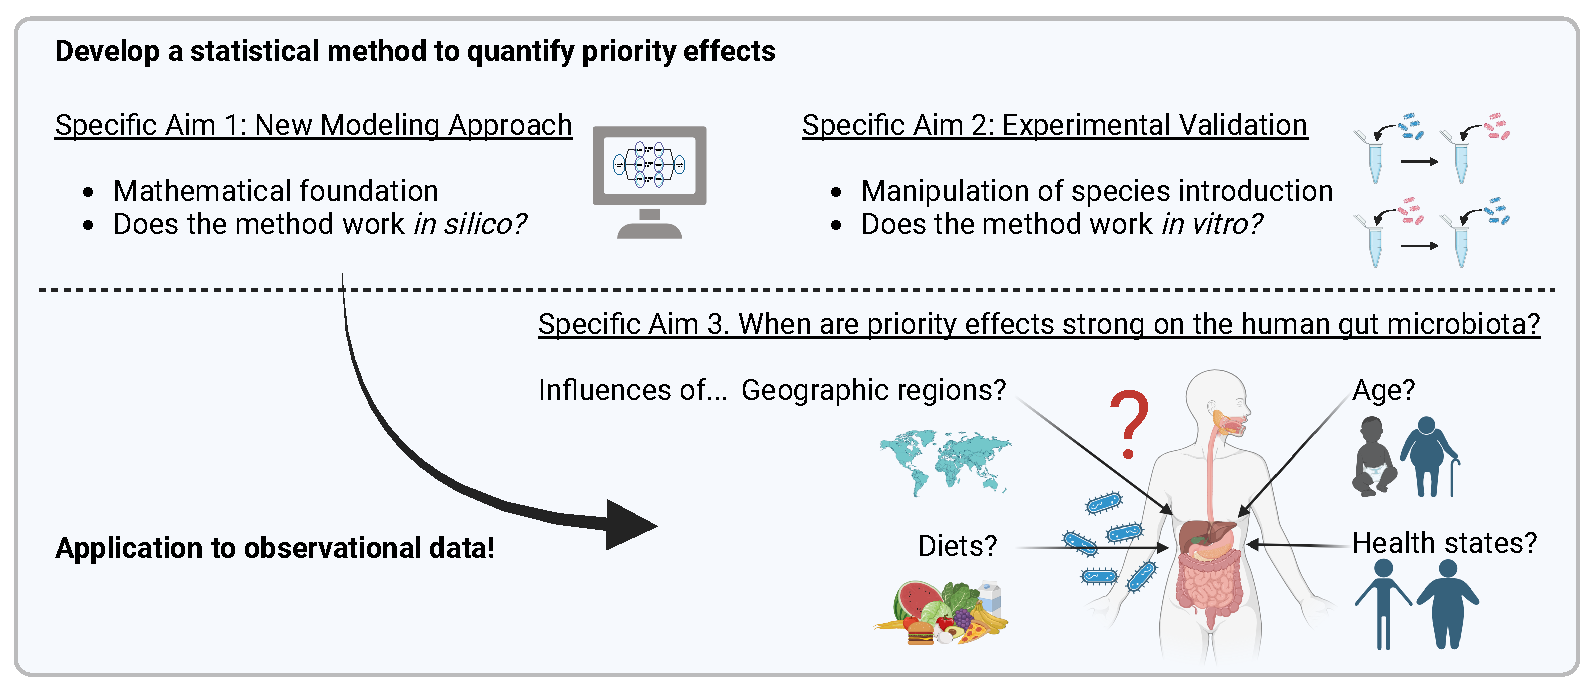
\includegraphics[scale=0.7]{output/figure_overview.pdf}
    \caption{Caption}
    \label{fig:overview}
\end{figure}

\section{Innovation}
Our proposed work will advance the fundamental understanding of the human microbiota and its relation to human health through a novel application of ecological theory to existing clinical data.
We believe this work is innovative both methodologically and conceptually for the following reasons.

First, \ul{\emph{it is methodologically innovative}} because the proposed method will be robust to the complexity of the microbiota.
A major challenge in community assembly research is the ``\textit{curse of dimensionality}.''
Namely, as the number of species increases, the non-linear system dynamics quickly become so complicated that traditional statistical approaches are no longer applicable.
This problem is particularly serious in microbial systems because the taxonomic diversity is far beyond that of plants and animals.
To confront this challenge, the proposed method condenses community information into a manageable number of parameters, as detailed in Specific Aim 1 below. 
This unique simplification allows us to use ordinary statistics to quantify priority effects.

Second, \ul{\emph{our work is also conceptually innovative}} because our method will enable us to provide a novel answer to \textit{when priority effects are strong on the human microbiota.}
Much of the research in priority effects has relied on experimental manipulations of species arrival order, with limited scope due to logistical and ethical challenges.
Some hypotheses have been proposed regarding the potential role of priority effects in the human microbiome.
For example, the gut microbial communities of obese, undernourished, and healthy people are hypothesized to represent alternative stable states resulting from priority effects \citep{fierer_animalcules_2012}.
Yet rigorous tests of these hypotheses have been difficult. 
The new method we will develop will provide a way to infer priority effects using existing time series data, allowing for comparison across individuals of different states.

Hence, we suggest that this proposal has two innovative qualities meeting the NIH review criterion "\emph{Does the application challenge and seek to shift current research or clinical practice paradigms by utilizing novel theoretical concepts?}"

\section{Approach}

\subsection*{Specific Aim 1: Development of a New Modeling Approach}

To develop a new modeling approach that identifies communities sensitive to priority effects, we will perform two activities:
[1a] derive a mathematical foundation for a statistical method that identifies sensitive communities and [1b] validate the performance of the proposed method with numerical simulation experiments.

\subsubsection*{Activity 1a: Derive a theoretical foundation}

\textbf{\textit{Goal}} -- 
Our goal in this activity is to develop a mathematical foundation for a statistical method that identifies sensitive communities.
In communities of interacting species, their sensitivity to priority effects is largely determined by the balance between intraspecific and interspecific competition, which are defined as the per-capita impact on population growth over time \citep{chesson_mechanisms_2000, barabas_chessons_2018, ke_coexistence_2018, terui_intentional_2023}.
For example, in two-species communities, the community is sensitive to priority effects if interspecific competition exceeds intraspecific competition \citep{ke_coexistence_2018}.
Therefore, the first step is to obtain reliable estimates of competition from an empirical time series.
However, in empirical settings, it is often infeasible to estimate those parameters because of the ``\textit{curse of dimensionality}:'' as the number of species $S$ in the community increases, the length of the time series required for estimation increases exponentially \citep{ovaskainen_how_2017}.
Here, we propose a robust statistical method that bypasses the curse of dimensionality. Specifically, \ul{our proposed method estimates the balance of intra- and interspecific competition, \textbf{\textit{regardless of the number of species}}, by capitalizing on the fact that species-level competition can be condensed into an aggregate effect of the total community density}.

Importantly, the application of this framework focusing on competitive interactions is not limited to communities where species interact only via resource competition.
In the following theoretical analysis, competition is defined and treated broadly, encompassing any net negative interaction between species.
Negative interactions can come not just from resource competition as strictly defined, but also from other types of interactions that characterize human-associated microbial communities, such as competition for space, interference via toxin production, and interspecific quorum sensing.

\textbf{\textit{Method detail: theoretical backbone}} -- 
We consider a discrete recursion equation to describe community dynamics over time. The population density of species $i$ at time $t$, $x_{t,i}$ is modeled as:

\begin{equation}
\label{eq:m0}
x_{t + 1, i} = x_{t, i} f(\overset{\rightarrow}{x}_{t}).
\end{equation}

$f(\cdot)$ is the function defining the per-capita population growth rate, and $\overset{\rightarrow}{x}_{t}$ represents a vector of population densities of potential competitors ($\overset{\rightarrow}{x}_{t} = \{x_{t,1}, x_{t,2}...x_{t,i},...,x_{t,S}\}$, where $S$ is the number of species).
Although the method we propose here applies to any functions that assume linear combinations of species interaction terms, let us use a Ricker model as a commonly used example \citep{ricker_stock_1954, fowler_species_2012, terui_intentional_2023}:

\begin{equation}
\label{eq:ricker}
f(\overset{\rightarrow}{x}_{t}) = \exp(r_i - \alpha_i x_{t,i} - \sum_{j \ne i} \beta_{ij} x_{t,j}),
\end{equation}

where $r_i$ is the intrinsic population growth, and $\alpha_{i}$ and $\beta_{ij}$ the intra- and interspecific competition coefficients.
The parameter $\beta_{ij}$ has a sample mean ($\mu_{\beta}$) and standard deviation ($\sigma_{\beta}$), assuming that they are drawn from a given probability distribution. 
Denoting the total community density as $X_t$ ($X_t = \sum_i x_{t,i}$) and re-parameterizing the interspecific competition $\beta_{ij}$ as $b_{ij} = (\beta_{ij} - \mu_{\beta}) \sigma_{\beta}^{-1}$, Equation \ref{eq:m0} can be reorganized as:

\begin{equation}
\label{eq:rickermod0}
f(\overset{\rightarrow}{x}_{t}) = \exp\left[r_i - (\alpha_i - \mu_{\beta} - \sigma_{\beta} \phi_i) x_{t,i} - (\mu_{\beta} +  \sigma_{\beta} \phi_i) X_t + e_{t,i} \right],
\end{equation}

where parameters $\phi_{i}$ and $e_{t,i}$ are the functions of $b_{ij}$: $\phi_i = (S-1)^{-1}\sum_{j \ne i} b_{ij}$ and $e_{t,i} = \sigma_{\beta} (S - 1) \mbox{cov}(b_{ij}, x_{t,j})$ [$\mbox{cov}(\cdot)$ denotes covariance].
The parameter $e_i$ may have a non-zero mean over time depending on the covariance.
Thus, it can be decomposed into the constant ($\overline{e}_i$) and stochastic components ($\xi_{t,i}$) as $e_{t,i} = \overline{e}_i + \xi_{t,i}$.
Writing $g_{i} = r_i + \overline{e}_i$, this re-formulation leads to:

\begin{equation}
\label{eq:rickermod}
    f(\overset{\rightarrow}{x}_{t}) = \exp\left[g_{i} - (\alpha_i - \mu_{\beta} - \sigma_{\beta} \phi_i) x_{t,i} - (\mu_{\beta} +  \sigma_{\beta} \phi_i) X_t + \xi_{t,i} \right].
\end{equation}

The original function (Equation \ref{eq:ricker}) parameterized competition effects by species and, therefore, requires $S$ parameters of competition.
In contrast, the re-organized function (Equation \ref{eq:rickermod}) has only two variables ($x_{t,i}$ and $X_t$), and the competition effects are condensed into the aggregate parameters of species $i$'s density ($\alpha_i - \mu_{\beta} - \sigma_{\beta} \phi_i$) and the total community density ($\mu_{\beta} + \sigma_{\beta} \phi_i$).
\ul{This re-parameterization enables statistical inference of interspecific competition even with relatively short time series data}.
Let $\gamma_i$ and $\delta_i$ be the standardized effects of $i$'s population density and the total community density, respectively ($\gamma_i = (\alpha_i - \mu_{\beta} - \sigma_{\beta} \phi_i)g_i^{-1}$ and $\delta_i = (\mu_{\beta} + \sigma_{\beta} \phi_i)g_i^{-1}$).
Then, the log-transformed per-capita growth rate $\ln f(\overset{\rightarrow}{x}_{t})$ becomes the following linear model:

\begin{equation}
\label{eq:rickerlog}
    \ln f(\overset{\rightarrow}{x}_{t}) = g_i (1 - \gamma_i x_{t,i} - \delta_i X_t) + \varepsilon_{t,i},
\end{equation}

where $\varepsilon_{t,i}$ is random environmental noise plus $\xi_{t,i}$, which can be modeled as a stochastic term in statistical inference. This re-parameterization greatly reduces the number of competition parameters ($S \rightarrow 2$), \ul{regardless of the number of species in the community}.

\textbf{\textit{Method detail: null model analysis}} --
The community's sensitivity to priority effects is affected by the balance between intra- and interspecific competition: when interspecific competition exceeds intraspecific competition, the community is sensitive to priority effects \citep{ke_coexistence_2018}.
An intuitive statistical method would be to compare the effects of $x_{t,i}$ ($\gamma_i$) and $X_t$ ($\delta_i$) on $i$'s population growth (see Equation \ref{eq:rickerlog}).
However, this comparison is inappropriate because we cannot statistically separate the effect of intra- and interspecific competition (see Equation \ref{eq:rickermod}).
We need an alternative approach to measure the balance of competition strength.

Here, \ul{we propose to use a neutral community as a reference to measure the sensitivity to priority effects.} 
A neutral community is comprised of ecologically identical species (intraspecific competition = interspecific competition) \citep{hubbell_unified_2001, loreau_species_2008}.
If the observed effect of $\delta_i$ is stronger than what would be expected from the hypothetical neutral dynamics, the community should be sensitive to priority effects.
Our proposed method has three steps:

\begin{enumerate}
    \item Estimate $\delta_i$ by fitting a linear statistical model to the observed population growth (see Equation \ref{eq:rickerlog}).
    We refer to this observed estimate as $\delta_{obs}$.
    While $\delta_{obs}$ can be estimated for each species, we will average across species to reduce the uncertainty of parameter estimate.
    
    \item Estimate $\delta_i$ for a hypothetical neutral community, which we refer to as $\delta_{null}$.
    Under the hypothetical neutral scenario, all species obey the same recursion equation with identical parameters ($g_i = \mbox{const.}$, $\alpha_i = \beta_{ij} = \mbox{const.}$), leading to the following dynamics of the total community density $X_t$: 

    \begin{equation}
    \label{eq:neutral}
        \ln f(X_t) &= \ln {X_{t+1}} - \ln {X_{t}} = g'(1 - \delta_{null} X_{t})        
    \end{equation}
    
    As such, $\delta_{null}$ can be readily estimated with ordinary regression using the observed data of $X_t$.
    
    \item Approximate the probability of $\delta_{obs} > \delta_{null}$.
    We will take a Bayesian approach to estimate a posterior distribution of $\delta_{obs}$.
    The approximated probability will be calculated as the proportion of posterior samples satisfying $\delta_{obs} > \delta_{null}$, and we refer to it as the \textbf{\textit{competitive exceedance}} $\Psi$ ($\approx \Pr(\delta_{obs} > \delta_{null})$).
\end{enumerate}

Our method can also be viewed as a variant of invasion analysis \citep{otto_biologists_2011}, with which ecologists study the coexistence of competing species \citep{chesson_mechanisms_2000, adler_niche_2007, barabas_chessons_2018}.
When multiple species satisfy the condition of $\delta_i > \delta_{null}$, one cannot invade the community when the other competitor(s) are already present.
Thus, priority effects should emerge (the invasion criterion $\delta_i > \delta_{null}$ can be derived from the Jacobian of Equations \ref{eq:rickermod} and \ref{eq:neutral}).

\subsubsection*{Activity 1b: Simulation experiment}

\textbf{\textit{Goal}} -- 
The goal of this activity is to validate the performance of this method using simulation experiments.
We will use time series data simulated with known parameters so that we can validate the relationship between the true sensitivity to priority effects and competitive exceedance $\Psi$.

\textbf{\textit{Method detail: preliminary analysis}} -- 
To validate the performance of the proposed null model analysis, we need to know whether the simulated data are generated from an insensitive or sensitive community (= the truth).
In two species Lotka-Volterra systems, priority effects emerge when interspecific competition exceeds intraspecific competition \citep{ke_coexistence_2018}.
However, for multi-species communities, the community dynamics are more complicated, especially when the strength of interspecific competition varies among species pairs \citep{carroll_niche_2011, barabas_chessons_2018}.

To address this complexity, we will use the leading eigenvalue $\lambda_{max}$ of the community matrix (the Jacobian of Equation \ref{eq:m0}) to determine whether the simulated community is sensitive to priority effects \citep{otto_biologists_2011}.
When the leading eigenvalue satisfies $|\lambda_{max}| < 1$, the community's equilibrium is locally stable and hence no priority effects.
Otherwise ($|\lambda_{max}| > 1$), the community's equilibrium is locally unstable with the possibility of priority effects.
We acknowledge that the criterion of $|\lambda_{max}| > 1$ is a necessary, not sufficient, condition for a priority effect to emerge.
Yet, it is reasonable to assume that such communities are sensitive to priority effects as the equilibrium condition is locally unstable  \citep{otto_biologists_2011}. 

Using this sensitivity criterion, we performed a preliminary analysis of the method's performance.
We used the model formula presented in Equation \ref{eq:ricker} (a Ricker model) to produce simulated time series data.
We considered 1782 combinations of demographic parameters to yield a sufficient variation in the leading eigenvalue $|\lambda_{max}|$ (Table \ref{tab:param1}).
We identified parameter combinations that generated insensitive and sensitive communities by calculating the leading eigenvalue for each parameter combination, after which 200 parameter sets were randomly subsampled to ensure that the relative frequencies of sensitive and insensitive communities were equal (100 sets have $|\lambda_{max}| < 1$ otherwise $|\lambda_{max}| > 1$).
We crossed these parameter sets with the number of species $S$ ($S \in \{2, 5, 10\}$) and the time series length $T$ ($T \in \{10, 30\}$) with five replicates in each, resulting in $200 \times 3 \times 2 \times 5 = 6000$ simulation runs.

\begin{SCfigure}
    \caption{Competitive exceedance $\Psi$ ($y$-axis) captures the critical transition from insensitive to sensitive communities, which are determined by the leading eigenvalue $\lambda_{max}$ ($x$-axis) of the community matrix (i.e., sensitive if $|\lambda_{max}| > 1$).
    The rows and columns distinguish the number of species and the time series length used to generate simulated data.
    Dots are individual simulation replicates with colors distinguishing the community's sensitivity to priority effects (orange: sensitive, blue: insensitive).}
    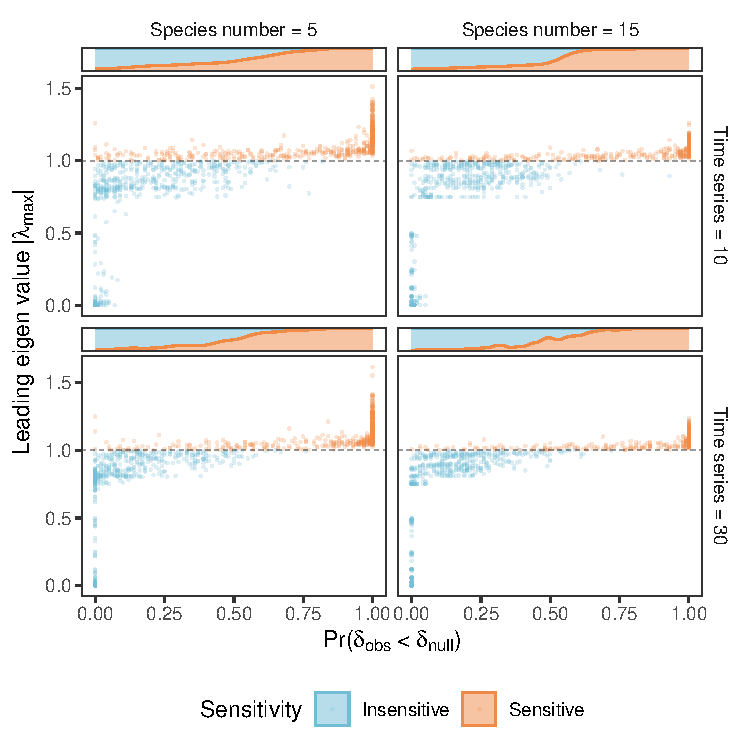
\includegraphics[scale=0.65]{output/figure_eigen_scatter.pdf}
    \label{fig:box}
\end{SCfigure}

The results of the preliminary analysis are promising.
\ul{The competitive exceedance $\Psi$ captured the critical transition from insensitive to sensitive communities} (Figure \ref{fig:box}).
The number of species did not have any noticeable effect on the performance of the proposed method.
Moreover, the performance was reasonable with a relatively short time series ($t = 10$).
These results indicate that our method can be effective even with short time series data from species-rich communities. 


\begin{table}
    \flushleft
    \caption{Possible parameter values in the proposed and preliminary analysis. In the proposed analysis, we will repeat the analysis across Ricker and Beverton-Holt models to simulate community dynamics. Note that intrinsic growth $r_i$ was/will be determined as $A \overset{\rightarrow}{x^*}$, where $\overset{\rightarrow}{x^*}$ is a vector of equilibrium densities and $A$ is an interaction matrix whose diagonal and off-diagonal elements are $\alpha_i$ and $\beta_{ij}$.
    The notation ``--'' means that we will use the same parameter setup in the proposed work.}
    \begin{tabular}{clll}
        Symbol & Interpretation & Value (preliminary) & Value (proposed)\\
        \hline
        $x^*$ & Average equilibrium density & $2, 8, 32$ & $1~\mbox{to}~100$\\
        $h_x$ & Half range in $x^*$ & $x^* \times 0.00~\mbox{to}~0.50$ & $x^* \times 0.00~\mbox{to}~1.00$\\
        $x_i^*$ & Equilibrium density for species $i$ & $\mbox{Unif}(x^* - h_x, x^* + h_x)$ & --\\
        $\alpha_{i}$ & Intraspecific competition & $1 / x^*$ & -- \\
        $\beta_{ij}$ & Interspecific competition & $\mbox{Unif(\mu_{\beta} - h_{\beta}, \mu_{\beta} + h_{\beta})}$ & -- \\
        $\mu_{\beta}$ & Average interspecific competition & $\alpha_i \times 0.00~\mbox{to}~2.00$ & --\\
        $h_{\beta}$ & Half range in $\beta_{ij}$ & $\mu_{\beta} \times 0.00~\mbox{to}~0.50$ & $\mu_{\beta} \times 0.00~\mbox{to}~1.00$ \\
        $r_i$ & Intrinsic population growth & $A \overset{\rightarrow}{x^*}$ & --\\
        \hline
    \end{tabular}
    \label{tab:param1}
\end{table}

\textbf{\textit{Method detail: proposed analysis}} -- 
Building on the preliminary analysis, we propose to expand the scope of simulation experiments to further evaluate the credibility of our method in a broader range of ecological situations.
Specifically, we will extend our analysis in two ways.

(i) \ul{Alternative theoretical model}:
Ecological systems can exhibit a diversity of competitive interactions.
We will consider alternative community models to capture different manners in which competitive community dynamics can be described. 
A Beverton-Holt (BH) model is a model widely used in ecology \citep{otto_biologists_2011}, describing the temporal dynamics of competitive communities: $\ln f(\overset{\rightarrow}{x}_{t}) = r_i - \ln(1 + \alpha_i x_{t,i} + \sum_j \beta_{ij} x_{t,j})$. 
While the model formula is different, a BH model shares one key feature with a Ricker model, that is, the linear combination of competitive interaction terms.
Hence, as in a Ricker model, a BH model can be simplified as follows: $\ln f(\overset{\rightarrow}{x}_{t}) \approx g'_{i} - \ln(1 + \gamma'_i x_{t,i} + \delta'_i X_t) + \varepsilon_{t,i}$ (see Box 1 for derivation).
This formulation indicates that the statistical inference of the key parameter ($\delta_i$) is possible through the fitting of a non-linear model.
We will use \texttt{stats::nls()} function in \texttt{R} or Bayesian models (e.g., Just Another Gibbs Sampler \citep{plummer_jags_2003}) to fit a non-linear model to the simulated data.

\begin{tcolorbox}[{
  breakable,
  colback=white,
  colframe=gray,
  coltext=black,
  parbox=false,
  boxsep=5pt,
  arc=1pt}]
    Box 1: Approximation of the Beverton-Holt model
    \hline
    In the Beverton-Holt (BH) model, the competition terms are modeled in a logarithmic scale as $\ln(1 + \alpha_i x_{t,i} + \sum_j \beta_{ij} x_{t,j})$.
    After the transformation outlined in the main text, this formula takes the form $\ln(1 + \gamma'_i x_{t,i} + \delta'_i X_t + e_{t,i})$, where $\gamma'_i = \alpha_i - \mu_{\beta} - \sigma_{\beta} \phi_i$ and $\delta'_i = \mu_{\beta} + \sigma_{\beta} \phi_i$.
    Here, to separate the nuisance term $e_{t,i}$ as an additive term in an ordinary scale, let us denote $c = 1 + \gamma'_i x_{t,i} + \delta'_i X_t$ and consider the Taylor series of $w(e_{t,i}) = \ln(c + e_{t,i})$ around $e_{t,i} = 0$:

    \begin{align}
        \begin{split}
        \label{eq:bhtaylor}
        w(e_i) &= \ln(c) + \frac{e_{t,i}}{c} - \frac{e_{t,i}^2}{2 c^2} + ...\\
        &\approx \ln(c) + O(e_{t,i}),
        \end{split}
    \end{align}

    where $O(e_{t,i})$ denotes the higher-order terms of the Taylor series necessary for proper approximation ($O(e_{t,i}) = \frac{e_{t,i}}{c} - \frac{e_{t,i}^2}{2 c^2} + ...$). 
    As a result, after accounting for environmental noise, the BH model can be approximated as:

    \begin{align}
    \begin{split}
        \ln f(\overset{\rightarrow}{x}_{t}) 
            &= r_i - \ln(1 + \alpha_i x_{t,i} + \sum_j \beta_{ij} x_{t,j})\\
            &= r_i - \ln(1 + \gamma'_i x_{t,i} + \delta'_{i} X_t + e_{t,j})\\
            &\approx g'_{i} - \ln(1 + \gamma'_i x_{t,i} + \delta'_i X_t) + \varepsilon_{t,i},
    \end{split}
    \end{align}

    where $g'_{i} = r_i + \overline{O(e_{t,i})}$.
    This form allows us to estimate the key parameter $\delta'_i$ through simple statistical inference.
\end{tcolorbox}

(ii) \ul{Broader parameter space}: We will expand the parameter space of the simulation experiment (Table \ref{tab:param1}) and increase the number of subsamples ($500~\mbox{to}~1000$ parameter combinations for each of insensitive and sensitive communities).
This broader parameter space will be crossed with two alternative theoretical models (Ricker and BH models) and a greater range of species richness ($S \in \{4, 8, 16, 32, 64\}$) and time series length ($T \in \{5, 10, 20, 40\}$).
Through this extended simulation experiment, we will confirm the usefulness of our method in broader ecological scenarios.

Collectively, these proposed activities will increase the credibility of our proposed method.

\subsection*{Specific Aim 2: Experimental Validation}

\textbf{\textit{Goal}} -- 
We aim to assess the performance of the proposed method using data from published experiments, in which species arrival history was manipulated.
While simulation experiments in Specific Aim 1 serve as the first step to assess the utility of our new method, Specific Aim 2 will allow us to evaluate the method's ability to predict priority effects when applied to real biological data.

\textit{\textbf{Method details: preliminary analysis}} --
We identified ten studies that manipulated species arrival history in a microbial community assembly experiment (Table \ref{tab:expdata}).
These data are ideal for our model validation for two reasons.
First, the results indicate that several species combinations show a strong sign of priority effects while other combinations do not.
Therefore, we can assess whether the competitive exceedance $\Psi$ predicts the strength of priority effects revealed in the experiments.
Second, these experiments vary in time series length and the number of species, allowing us to evaluate the robustness of our method. 
Most of the experiments listed in Table \ref{tab:expdata} involved free-living microbial systems consisting of freshwater bacteria, protists, and algae, but one of the experiments, Ojima et al. [21], used common species of \textit{Bifidobacterium} isolated from the human infant gut. 

\begin{table}
    \flushleft
    \caption{Published time series data of experimental communities.}
    \begin{tabular}{llll}
         Source & Study system & Time series length & \# species in a community\\
         \hline
         Fukami and Morin \citep{fukami_productivity-biodiversity_2003} & Protists & $6$ & $18$\\
         Fukami \citep{fukami_assembly_2004} & Protists & $10$ & $14$\\
         Price and Morin \citep{price_colonization_2004} & Protists & $\ge 20$ & $2$ or $3$ \\
         Zhang and Zhang \citep{zhang_colonization_2007} & Algae & $13$ & $2$\\
         Jiang and Patel \citep{jiang_community_2008} & Protists & $7$ & $10$\\
         Tucker and Fukami \citep{tucker_environmental_2014} & Bacteria and yeasts & $9$ & $4$\\
         Pu and Jiang \citep{pu_dispersal_2015} & Protists & $13$ & $10$\\
         Ojima and Jiang \citep{ojima_interactive_2017} & Protists & $23$ & $5$\\
         Hsu and Moeller \citep{hsu_metabolic_2021} & Protists & $13~\mbox{to}~22$ & $2$\\
         Ojima et al. \citep{ojima_priority_2022} & Bacteria & $7$ & $2$ or $4$\\
         \hline
    \end{tabular}
    \label{tab:expdata}
\end{table}

We applied our method to the datasets in Hsu and Moeller \citep{hsu_metabolic_2021} and Ojima \textit{et al.} \citep{ojima_priority_2022}, serving as a preliminary application to real biological data.
In their experiments, the authors manipulated the introduction order of competing species (two species of bacterivorous ciliates in Hsu and Moeller \citep{hsu_metabolic_2021} and four species of bifidobacteria in Ojima \textit{et al.} \citep{ojima_priority_2022}) to quantify the strength of priority effects.
A pair of species were introduced into an experimental medium with different introduction timings (simultaneous, species 1 first, or species 2 first), and temporal changes of species densities were measured at multiple time points (seven to 22 time points).
Their results indicated that the strength of priority effects, as quantified by the method proposed by Vannette and Fukami \citep{vannette_historical_2014}, varied with light conditions \citep{hsu_metabolic_2021} or species combinations \citep{ojima_priority_2022}.
Hence, these data are an ideal test case for our proposed method.

Our analysis proceeded as follows:

\begin{enumerate}
    \item Select the appropriate ecological model.
    We fitted Ricker and BH models to the empirical time series and estimated Akaike's Information Criterion (AIC) \citep{burnham_model_2002} for each model.
    In the following analysis, we used the model with a lower AIC value (a Ricker model, in this case).
    \item Perform the null model analysis to obtain competitive exceedance $\Psi$.
    We analyzed time series data after both species were introduced.
    Thus \textit{no information on arrival history was given to the analysis}.
    \item Validate the relationship between the strength of priority effects (known as the experiment outcome) and competitive exceedance $\Psi$.
    We used Vannette and Fukami's method \citep{vannette_historical_2014} to quantify the experimentally estimated strength of priority effects.
    This method calculates priority effect strength as the absolute log-response ratio $LRR = |\ln (D_{1, max} / D_{2, max})|$, where $D_{1, max}$ and $D_{2, max}$ are the maximum species density when they were introduced first and second, respectively \citep{hsu_metabolic_2021}.
    The greater values of $LRR$ indicate stronger priority effects (either inhibitory or facilitative), but \textit{this metric cannot be estimated unless we manipulate the order of species introduction}.
    We examined how well competitive exceedance $\Psi$ predicts $LRR$.
\end{enumerate}

\begin{wrapfigure}{r}{0.35\textwidth}
    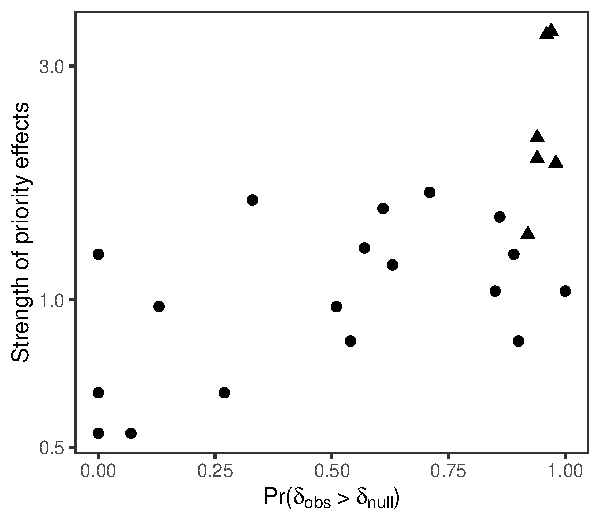
\includegraphics[scale=0.6]{output/figure_exp.pdf}
    \caption{The competitive exceedance $\Psi$ predicts the strength of priority effects in experimental communities (data from Hsu and Moeller \citep{hsu_metabolic_2021} and Ojima et al. \citep{ojima_priority_2022}).
    Each data point represents an individual time series, and symbol shapes distinguish data sources (circle = Hsu and Moeller, triangle = Ojima et al.)}
    \label{fig:experiment}
\end{wrapfigure}

As expected from our preliminary simulation experiments, competitive exceedance $\Psi$ predicted the strength of priority effects $LRR$ reasonably well (Figure \ref{fig:experiment}).

\textit{\textbf{Method details: proposed analysis}} --
We will conduct this analysis for the rest of the experimental data listed in Table \ref{tab:expdata}.
In addition, we will search for additional published experimental data to broaden the taxonomic scope of our validation.

In the expanded analysis, we will use metrics of community dissimilarity between treatments with different introduction orders to quantify the strength of priority effects.
Although $LRR$ is an intuitive measure for quantifying priority effects in species pairs, priority effects on communities consisting of more than two species can be better captured by overall community dissimilarity.
Thus, we will quantify the extent of community dissimilarity for all pairs of introduction history, and use the average of those values as the strength of priority effects.

For this analysis, we will use two metrics of community similarity, the Morisita-Horn index and the Bray-Curtis index.
The advantage of the Morisita-Horn index is that it quantifies community similarity based on the relative abundance \citep{magurran_biological_2011}, making it possible to compare among experimental systems that can vary greatly in absolute abundances.
On the other hand, similarity based on relative abundance can be difficult when differences in absolute abundance are also of interest in comparing communities.
Unlike the Morisita-Horn index, the Bray-Curtis index is sensitive to differences in absolute abundances\citep{magurran_biological_2011}.

Our proposed analysis will allow us to answer the following two questions, which will help better clarify the strengths and limitations of our proposed method.
(i) Does our method's performance vary by time series length and/or the number of species?
(ii) Does our method's performance vary by taxonomic group?
We expect our method to be robust in terms of (i) and (ii), in light of the results of the preliminary simulation experiments.
Nevertheless, we will study the cases where the method's performance turns out to be relatively poor.
We will use this analysis to explore how our method can be further refined.

\subsection*{Specific Aim 3: Application to Unmanipulated Systems}

\textbf{\textit{Goal}} -- 
We aim to assess and identify factors that contribute to priority effects in human gut microbes.
Having confirmed the validity of our proposed methods through Specific Aims 1 and 2, we will now be ready to apply the method to observational data on the human gut microbiome to ask questions that will inform us when to expect strong priority effects.

\textit{\textbf{Method details: data source}} --
We will use published time series data of human gut microbiomes.
The following keywords will be used to search the literature (title, abstract, or keywords fields) that may contain the time series data: ``\textit{human* gut* microb* `time series' OR `longitudinal'.}''
Our preliminary search in SCOPUS identified 202 articles (as of 1/10/24), serveral of which contained promising data.
For example, Vandeputte et al. 2021 \citep{vandeputte_temporal_2021} performed daily quantitative microbiome profiling on 713 fecal samples from 20 Belgian women over six weeks, combined with extensive anthropometric measurements, blood panels, dietary data, and stool characteristics. 
We will verify the data quality of each time series with the following inclusion criteria: (i) the length of the consecutive time series exceeds four-time points; (ii) the entire community members are collected; (iii) absolute quantitative data are available; and (iv) the sampling method is consistent across the time series.
For those that meet the inclusion criteria, we will apply the following time-series analysis to estimate competition parameter $\delta_{obs}$.

\textit{\textbf{Method details: time series analysis}} --
Unlike simulated and experimental time series data, observational data may contain substantial observation errors.
We will employ a Bayesian state-space model to account for observation errors \citep{kery_bayesian_2012, amano_hierarchical_2012, anderson_black-swan_2017, terui_metapopulation_2018, terui_intentional_2023}.
The Bayesian state-space model is one of the time series models and has proven to provide less-biased estimates of critical demographic parameters from noisy data \citep{kery_bayesian_2012}.

The observed density of species $i$ at time $t$, $N_{t,i}$, will be modeled as random draws from a log-normal distribution: $\ln N_{t,i} \sim \mbox{Normal}(x_{t,i}, \sigma_{obs}^2).$
The mean parameter $x_{t,i}$ is the latent variable that represents ``true'' species density (abundance per unit effort) and the standard deviation $\sigma_{obs}$ measures stochastic observation errors.
We will also be able to account for systematic observation errors if the information is available as covariates (e.g., sampling protocol).
Thus, this modeling framework allows for robust statistical inference \citep{kery_bayesian_2012}.

Either a Ricker or BH model will be fitted to the latent density $x_{t,i}$ to estimate species-specific $\delta_i$: $\ln x_{t + 1,i} &= \ln x_{t,i} + \ln f(\overset{\rightarrow}{x}_{t}) + \varepsilon_{t,i}$, where $\varepsilon_{t,i}$ is a normal error term with standard deviation $\sigma_{state}$ measuring the degree of stochastic environmental noise.
Hierarchical modeling allows us to estimate the mean competition parameter averaged across species ($\hat{\delta}_{obs}$) as a hyper-parameter of $\delta_i$: i.e., $\delta_i \sim \mbox{Normal}(\hat{\delta}_{obs}, \sigma^2_{\delta})$.
We will calculate competitive exceedance $\Psi$ as $\Pr(\hat{\delta}_{obs} > \delta_{null})$.

\textit{\textbf{Method details: drivers of priority effects}} --
We will analyze factors influencing competitive exceedance $\Psi$ in the human gut microbiome to gain insights into the prevalence of gut microbial communities sensitive to priority effects and individual attributes contributing to the sensitivity to priority effects.
To this end, we will leverage the individual replicates of $\Psi$.
To properly model $\Psi_k$ for individual $k$, our basic model will take the number of posterior samples that satisfy $\hat{\delta}_{k,obs} > \delta_{null}$ for individual $k$ ($Y_k$) as a response variable: $Y_k &\sim \mbox{Binomial}(N_{post}, P_k)$, where $N_{post}$ is the total number of posterior samples.
Thus, the success probability of the binomial distribution $P_k$ is identical to competitive exceedance $\Psi_k$, which we will relate to linear predictors: $\mbox{logit}(\Psi_k) &= \theta_0 + \sum_q \theta_q z_{q,k}$.
The parameter $\theta_0$ is the intercept, and $\theta_q$ the $q$-th regression coefficient quantifying the influence of the predictor $z_{q,k}$.
The predictors $z_{q,k}$ will include individual attributes that could contribute to the sensitivity to priority effects. 
Using this modeling framework, we will address four hypotheses: (i) Does the strength of priority effects vary across geographic regions?
(ii) Do Western-style diets influence the strength of priority effects?
(iii) Are priority effects stronger at younger ages?
(iv) Are priority effects stronger in individuals with unhealthy states?


\ul{[Hypothesis \textit{i}] \textit{Does the strength of priority effects vary across geographic regions?}} 
The likelihood of priority effects may depend on potential colonists in the environment since priority effects stem from mutual non-invasibility between certain combinations of species \citep{fukami_historical_2015}.
Cultural habits differ substantially across geographic regions, and such differences are thought to create variation in the species pool of microbial communities \citep{de_filippo_impact_2010, yatsunenko_human_2012, david_host_2014}.
Therefore, different geographic regions may experience varied strengths of priority effects.
We will evaluate the difference in competitive exceedance $\Psi$ by country because it is linked to cultural differences \citep{yatsunenko_human_2012}.

\ul{[Hypothesis \textit{ii}] \textit{Do Western-style diets influence the strength of priority effects?}}
Diet is an important determinant of gut microbial communities \citep{de_filippo_impact_2010, yatsunenko_human_2012, schnorr_gut_2014, zimmer_vegan_2012, smits_seasonal_2017}.
In particular, many studies found shifts in gut microbiota between Western and non-Western populations with health outcomes, and these shifts were attributable to changes in dietary fat \citep{reese_thinking_2019}.
Different sets of species may be prevalent between populations with Western and non-Western dietary habits, likely leading to varied strengths of priority effects. 
We will assess the difference in $\Psi$ between populations with Western and non-Western diets by re-classifying countries based on dietary habits \citep{kariel_proposed_1966}.

\ul{[Hypothesis \textit{iii}] \textit{Are priority effects stronger at younger ages?}}
Anecdotal evidence suggests that priority effects are stronger at younger ages.
For example, an infant's gut microbiota is strongly influenced by delivery mode (vaginal vs caesarean section) and feeding regime (formula vs breastmilk) \citep{bokulich_antibiotics_2016, akagawa_effect_2019, dominguez-bello_delivery_2010}, implying the manifestation of priority effects.
In contrast, adult gut microbiota has been hypothesized to be in a stable climax state \citep{fierer_animalcules_2012, costello_application_2012}, although supporting evidence for this claim is limited \citep{fierer_animalcules_2012}.
We therefore hypothesize that priority effects are stronger at younger ages.
We will yield the subject's age or age-class information from data sources and examine whether competitive exceedance $\Psi$ changes with age.

\ul{[Hypothesis \textit{iv}] \textit{Are priority effects stronger in individuals with unhealthy states?}}
Dysbiosis is often associated with unhealthy states \citep{petersen_defining_2014, fierer_animalcules_2012}, and it was hypothesized that these reflect alternative stable states resulting from priority effects \citep{fierer_animalcules_2012}.
However, this hypothesis has not been tested because of the lack of proper statistical methods.
Here, we will utilize competitive exceedance $\Psi$ as a proxy for priority effects and will compare this value between healthy and unhealthy people (IBD and/or obesity).
If unhealthy people harbor microbial communities sensitive to priority effects, they should show higher values of $\Psi$.

When we test these hypotheses, we will include potential covariates in the model to statistically control influences of possible confounding factors.
Such factors may include, but are not limited to, sex, sampling methods (if multiple methods are employed), time-series length, and/or study ID.
The inclusion of covariates is necessary to yield less biased estimates of the primary factor's effects.

\subsection*{Outlook}
While our focus in this proposal is the gut system, we expect our proposed method will create opportunities for understanding the assembly of microbial communities in or on other parts of the human body, such as the skin and the oral cavity.
These microbial communities also mediate human health \citep{fierer_animalcules_2012}.
The increasing attention to their health consequences stimulated researchers to study the underlying mechanisms of community assembly \citep{grice_topographical_2009, jakobsson_short-term_2010, costello_bacterial_2009, caporaso_moving_2011}.
They share some characteristics with gut microbial communities, despite substantial differences in the identity of constituent species \citep{costello_bacterial_2009}.
At the same time, microbes inhabiting different parts of the human body show contrasting patterns in temporal compositional changes \citep{costello_bacterial_2009, caporaso_moving_2011, fierer_animalcules_2012, jakobsson_short-term_2010}.
Oral cavity communities show greater stability in community structure over time with persistent core species, while the skin harbors more transient species with frequent changes in species dominance and composition \citep{costello_bacterial_2009}.
These observations suggest that different assembly rules among body sites, likely with varied strengths of priority effects.
Time-series data have continued to accumulate on these systems, to which our new method should be applicable.

\begin{table}
    \centering
    \caption{Project time table}
    \begin{tabular}{lccccc}
         & Y1 &  Y2 & Y3 & Y4 & Y5\\
         \hline
         Aim 1 & Method refinement & Package development & & & \\
         Aim 2 & Assemble data & Experimental validation (EV) & EV &  & \\
         Aim 3 & & Data compilation (DC) & DC & Data analysis (DA) & DA \\
    \end{tabular}
    \label{tab:tt}
\end{table}

\newpage

\bibliography{references}

\end{document}